% !TeX program = xelatex
\documentclass[notheorems]{beamer}
% \documentclass{beamer}

\mode<presentation>
{
  % \usetheme{default}
  \usetheme{Antibes}
  \setbeamertemplate{footline}[frame number]{}
  \setbeamertemplate{navigation symbols}{}
}

\usepackage{amsmath}
\usepackage{xeCJK}
\setCJKsansfont[ItalicFont={Microsoft YaHei}]{Microsoft YaHei}

% liangduan
\usepackage{ragged2e}
\justifying\let\raggedright\justifying

\makeatletter
\newenvironment<>{proofs}[1][\proofname]{
    \par
    \def\insertproofname{#1\@addpunct{.}}
    \usebeamertemplate{proof begin}#2}
  {\usebeamertemplate{proof end}}

  \newenvironment<>{solution}[1][Solution.]{
    \par
    \def\insertproofname{#1\@addpunct{.}}
    \usebeamertemplate{proof begin}#2}
  {\usebeamertemplate{proof end}}

  \newtheorem*{definition}{Definition}
  \newtheorem{example}{Example}[section]
  \newtheorem{theorem}{Theorem}[section]
  \newtheorem{property}{Property}[section]
\makeatother

\setbeamertemplate{theorems}[numbered]
% \setbeamertemplate{definition}[nonumbered]

\setbeamertemplate{section in toc}[sections numbered]
\setbeamertemplate{subsection in toc}[subsections numbered]
% \setbeamertemplate{subsubsection in toc}[subsubsections numbered]

\numberwithin{equation}{section}
\numberwithin{equation}{subsection}

\usefonttheme[onlymath]{serif}
\providecommand{\Arg}{\operatorname{Arg}}
\providecommand{\Ln}{\operatorname{Ln}}
\providecommand{\Arcsin}{\operatorname{Arcsin}}
\providecommand{\Arccos}{\operatorname{Arccos}}
\providecommand{\Arctan}{\operatorname{Arctan}}
\providecommand{\Arcsinh}{\operatorname{Arcsinh}}
\providecommand{\Arccosh}{\operatorname{Arccosh}}
\providecommand{\Arctanh}{\operatorname{Arctanh}}

% \providecommand{\abs}[1]{\lvert#1\rvert}
\providecommand{\abs}[1]{\left\lvert#1\right\rvert}
% \providecommand{\norm}[1]{\lVert#1\rVert}

\title{Chapter 1: Complex Numbers and \\ Complex Functions}
% \subtitle{Complex number and complex variable function}
\author{Taotao Wang, Associate Professor}
\institute{College of Electronics and Information Engineering, Shenzhen University}
% \date{\today}

\begin{document}

\everymath{\displaystyle}

\begin{frame}
  \titlepage
\end{frame}

\begin{frame}{Outline}
  \tableofcontents
  % You might wish to add the option [pausesections]
\end{frame}

%\section{Complex number and complex function}

\section{Complex Numbers and Their Expressions}

\begin{frame}
\frametitle{Outline}
\tableofcontents[currentsection] 
\end{frame}

\begin{frame}
  \begin{enumerate}
    \item {\bf The Concept of Complex Numbers} \\
          In the real number system, the equation $x^2=-1$ has no solution. To solve such equations, we introduce the imaginary unit（虚数单位） $i$ (often denoted by $j$ in electrical engineering), defined by $i^2=-1$. Thus, $i$ is a solution of $x^2=-1$.\\
          For any real numbers $x$ and $y$, the number $z=x+iy$ is called a complex number（复数）. The quantities $x$ and $y$ are the real part（实部） and imaginary part（虚部） of $z$, respectively, and are denoted by $x=\operatorname{Re}(z)$ and $y=\operatorname{Im}(z)$.
  \end{enumerate}
\end{frame}

\begin{frame}
  \begin{enumerate}
    \item []
          When the coefficient of $i$ is numerical, we usually write $i$ after the coefficient, as in $2+3i$. When the coefficient is a variable, we often write $i$ before it, as in $a+ib$.\\
          If $x=0$ and $y\neq0$, then $z=iy$ is called a purely imaginary number（纯虚数）. If $y=0$, then $z=x$, so every real number is naturally a complex number.
  \end{enumerate}
\end{frame}

\begin{frame}
  \begin{enumerate}
    \setcounter{enumi}{1}
    \item {\bf Expressions of Complex Numbers}\\     
          A complex number $z=x+iy$ is uniquely determined by the ordered pair（有序数对） $(x,y)$. Therefore, complex numbers are in one-to-one correspondence with points in a two-dimensional Cartesian coordinate system（二维直角坐标系）: the number $z=x+iy$ is represented by the point $(x,y)$.
          This plane is called the complex plane（复平面）, or the $z$-plane. The $x$-axis is called the real axis（实轴）, and the $y$-axis is called the imaginary axis（虚轴）.
          
  \end{enumerate}
\end{frame}

\begin{frame}
  \begin{enumerate}
    \item []
          Each complex number $z=x+iy$ determines exactly one point $(x,y)$ in the complex plane, and vice versa. This correspondence allows us to study complex functions using geometric language and methods, and it provides a geometric foundation for many engineering applications.
  \end{enumerate}
\end{frame}

\begin{frame}
  \begin{enumerate}
    \item []
          In the complex plane, $z=x+iy$ also corresponds to the position vector（位置向量） $\overrightarrow{OP}$ from the origin（原点） $O$ to the point $P=(x,y)$ (see Figure 1.1). This is the vector representation（向量表示） of $z$. The length of this vector is called the modulus（模）, or absolute value（绝对值）, of $z$ and is denoted by
          \[\abs{z}=r=\sqrt{x^2+y^2} \tag{1.1.1}\]
  \end{enumerate}
\end{frame}



\begin{frame}
\begin{enumerate}
	\item []
	\begin{figure}
		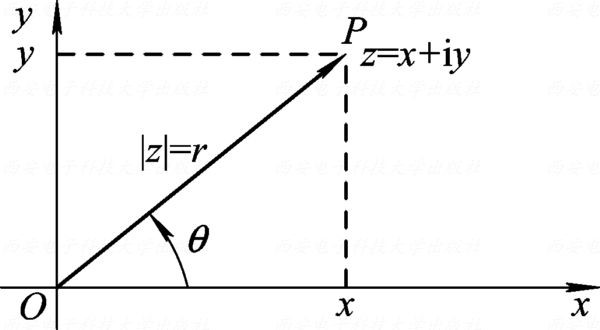
\includegraphics[height=0.6\textheight]{Figure_1_1.jpg}
		\caption{1.1}
	\end{figure}
\end{enumerate}
\end{frame}


\begin{frame}
\begin{enumerate}
	\item []
	The following inequalities are immediate:
	\[\abs{x}\leq\abs{z},\quad \abs{y}\leq\abs{z},\quad \abs{z}\leq\abs{x}+\abs{y}.\]
	For $z\neq0$, an angle $\theta$ measured counterclockwise（逆时针） from the positive real axis to the vector $\overrightarrow{OP}$ is called an argument（幅角） of $z$. Since $x=r\cos\theta$ and $y=r\sin\theta$, we have
	\[\tan\theta=\frac{y}{x}\quad(x\neq0). \tag{1.1.2}\]
\end{enumerate}
\end{frame}

\begin{frame}

\begin{enumerate}
	\item []
	Every nonzero complex number has infinitely many arguments (see Figure 1.2). If $\theta_1$ is one argument of $z$, then all its arguments are
    \[ \Arg z=\{\theta_1+2k\pi:k\in\mathbb{Z}\}. \tag{1.1.3} \]
	Here, $\Arg z$ denotes the set of all arguments of $z$.
\end{enumerate}

\end{frame}




\begin{frame}
\begin{enumerate}
	\item []
	\begin{figure}
		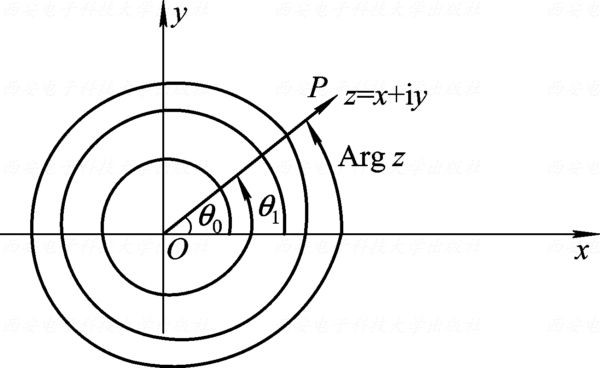
\includegraphics[height=0.6\textheight]{Figure_1_2.jpg}
		\caption{1.2}
	\end{figure}
\end{enumerate}
\end{frame}


\begin{frame}
\begin{enumerate}
	\item []
	Among all arguments of $z$, the unique value $\theta_0$ satisfying $-\pi<\theta_0\leq\pi$ is called the principal argument（幅角主值） and is denoted by $\arg z=\theta_0$. Hence,
	\[\Arg z=\{\arg z+2k\pi:k\in\mathbb{Z}\}. \tag{1.1.4}\]
	The argument of $z=0$ is undefined.
\end{enumerate}
\end{frame}

\begin{frame}
\begin{enumerate}
	\item []
	For $z=x+iy\neq0$, the principal argument can be determined from $\arctan(y/x)$ together with the quadrant（象限） of $z$:\\
	\resizebox*{\linewidth}{!}{
		\begin{minipage}{1.2\linewidth}
			\[\arg z(z\neq 0)=\begin{cases}
			\arctan\!\left(\frac{y}{x}\right)     & (z\text{ is in the 1st or 4th quadrant}) \\
			\arctan\!\left(\frac{y}{x}\right)+\pi & (z\text{ is in the 2nd quadrant})            \\
			\arctan\!\left(\frac{y}{x}\right)-\pi & (z\text{ is in the 3rd quadrant})             \\
			\frac{\pi}{2}            & (z\text{ is on the positive imaginary axis})    \\
			-\frac{\pi}{2}           & (z\text{ is on the negative imaginary axis})    \\
			\pi                      & (z\text{ is on the negative real axis})         \\
			0                        & (z\text{ is on the positive real axis})
			\end{cases}\tag{1.1.5}\]
		\end{minipage}
	}
\end{enumerate}
\end{frame}

\begin{frame}
\begin{enumerate}
	\item []
	\begin{figure}
		\centering
		\begin{minipage}{0.45\textwidth}
			\centering
			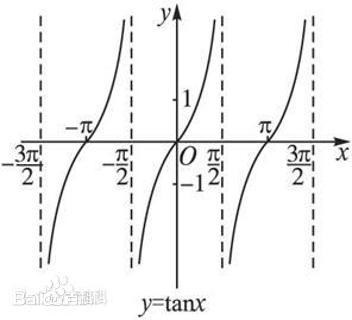
\includegraphics[width=1\textwidth]{Figure_1_2_a.jpg}
		\end{minipage}\hfill
		\begin{minipage}{0.45\textwidth}
			\centering
			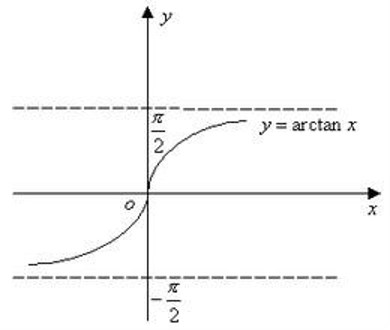
\includegraphics[width=1\textwidth]{Figure_1_2_b.jpg}
		\end{minipage}
	\end{figure}
\end{enumerate}
\end{frame}


\begin{frame}
\begin{enumerate}
	\item []
	\begin{figure}
		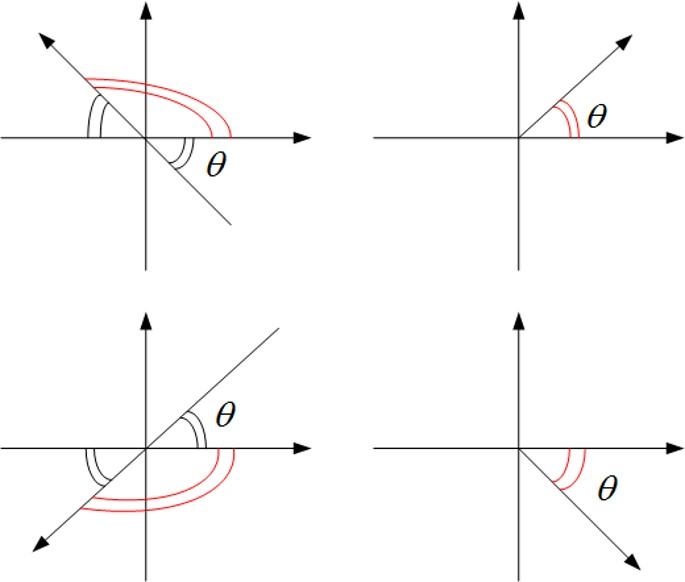
\includegraphics[height=0.8\textheight]{Figure_1_2_c.jpg}
	\end{figure}
\end{enumerate}
\end{frame}



\begin{frame}
\begin{example}
	Find all arguments and the principal argument of $1+i$ and $-3\sqrt{3}-3i$.
\end{example}
\begin{solution}<2->
	For $z=1+i$, the point lies in the first quadrant, so its principal argument is
	\[\arg z=\arctan\frac{y}{x}=\arctan1=\frac{\pi}{4}\]
	The arguments are given by
	\[\Arg z=\arg z+2k\pi=\frac{\pi}{4}+2k\pi\quad(k\in\mathbb{Z}).\]
\end{solution}
\end{frame}



\begin{frame}
\begin{solution}[Solution\ (Cont.)]
	For $z=-3\sqrt{3}-3i$, the point lies in the third quadrant, so its principal argument is
	\[\arg z=\arctan\frac{y}{x}-\pi=\arctan\frac{-3}{-3\sqrt{3}}-\pi=-\frac{5}{6}\pi.\]
	All its arguments are
	\[\Arg z=\arg z+2k\pi=-\frac{5}{6}\pi+2k\pi\quad(k\in\mathbb{Z}).\]
\end{solution}
\end{frame}


\begin{frame}
\begin{enumerate}
	\item []
	Using the relations between rectangular coordinates（直角坐标） and polar coordinates（极坐标）, $x=r\cos\theta$ and $y=r\sin\theta$, we can write
	\[z=r(\cos\theta+i\sin\theta) \tag{1.1.6}\]
    where $r$ is the modulus of $z$ and $\theta$ is any argument of $z$. This is called the trigonometric form（三角形式） of $z$.
\end{enumerate}
\end{frame}


\begin{frame}
\begin{enumerate}
	\item []
	Using Euler's formula（欧拉公式） $e^{i\theta}=\cos\theta+i\sin\theta$, the trigonometric form becomes
	\[z=re^{i\theta} \tag{1.1.7}\]
	This is called the exponential form（指数形式） of $z$. Because $\theta$ may be replaced by $\theta+2k\pi$, the trigonometric and exponential forms are not unique, even though they represent the same complex number.
\end{enumerate}
\end{frame}


\begin{frame}
\begin{example}
	Express $z=1+\sin1+i\cos1$ in trigonometric and exponential forms.
\end{example}
\begin{solution}<2->
	First compute the modulus $r$ and the principal argument $\arg z$:
	\begin{align*}
	r^2 & =(1+\sin1)^2+\cos^2 1=2(1+\sin1)                                                                \\
	& =2\left[1+\cos\left(\frac{\pi}{2}-1\right)\right]=4\cos^2\left(\frac{\pi}{4}-\frac{1}{2}\right) \\
	r   & =2\cos\left(\frac{\pi}{4}-\frac{1}{2}\right)>0
	\end{align*}
\end{solution}
\end{frame}


\begin{frame}
\begin{solution}[Solution\ (Cont.)]
	Since $1+\sin1>0$ and $\cos1>0$, the point $z$ lies in the first quadrant.
	\begin{align*}
	\arg z & =\arctan\frac{y}{x}=\arctan\left(\frac{\cos1}{1+\sin1}\right)
	\\
	& =\arctan\left[\frac{\sin\left(\frac{\pi}{2}-1\right)}{1+\cos\left(\frac{\pi}{2}-1\right)}\right]                                                                 \\
	& =\arctan\left[\frac{2\sin\left(\frac{\pi}{4}-\frac{1}{2}\right)\cos\left(\frac{\pi}{4}-\frac{1}{2}\right)}{2\cos^2\left(\frac{\pi}{4}-\frac{1}{2}\right)}\right] \\
	& =\left(\frac{\pi}{4}-\frac{1}{2}\right)
	\end{align*}
\end{solution}
\end{frame}

\begin{frame}
\begin{solution}[Solution\ (Cont.)]
	Therefore, the trigonometric form of $z$ is
	\[z=2\cos\left(\frac{\pi}{4}-\frac{1}{2}\right)\left[\cos\left(\frac{\pi}{4}-\frac{1}{2}\right)+i\sin\left(\frac{\pi}{4}-\frac{1}{2}\right)\right]\]
	Its exponential form is
	\[z=2\cos\left(\frac{\pi}{4}-\frac{1}{2}\right)e^{i\left(\frac{\pi}{4}-\frac{1}{2}\right)}\]
	When writing a trigonometric or exponential form, it is usually convenient to choose $\theta=\arg z$.
\end{solution}
\end{frame}


\begin{frame}
On the nonuniqueness of arguments:
\begin{enumerate}
	\item All arguments of $1+i$ are $\pi/4+2k\pi$, where $k\in\mathbb{Z}$;
	\item Its exponential forms are $\sqrt{2}e^{i(\pi/4+2k\pi)}$, all of which have the same value;
	\item Using the principal argument, we usually write the complex number simply as $\sqrt{2}e^{i\pi/4}$.
\end{enumerate}
\end{frame}




\section{Operations of Complex Numbers}


\begin{frame}
\frametitle{Outline}
\tableofcontents[currentsection] 
\end{frame}

\begin{frame}
\begin{enumerate}
	\item {\bf Four Arithmetic Operations of Complex Numbers}
	
	The sum and difference of two complex numbers $z_1=x_1+iy_1$ and $z_2=x_2+iy_2$ are defined by
	\[(x_1+iy_1)\pm(x_2+iy_2)=(x_1\pm x_2)+i(y_1\pm y_2) \tag{1.2.1}\]
	Thus, we add or subtract the real parts and imaginary parts separately. When $y_1=y_2=0$, these definitions reduce to the usual operations on real numbers.
\end{enumerate}
\end{frame}



\begin{frame}
\begin{enumerate}
	\item []
	Let $z_1$ and $z_2$ be represented by the vectors $\overrightarrow{OP_1}$ and $\overrightarrow{OP_2}$. Complex addition and subtraction agree with vector addition and subtraction. Hence, the diagonal（对角线） $\overrightarrow{OP}$ of the parallelogram（平行四边形） with adjacent sides（邻边） $\overrightarrow{OP_1}$ and $\overrightarrow{OP_2}$ represents $z_1+z_2$, while $\overrightarrow{P_2P_1}$ represents $z_1-z_2$ (see Figure 1.3).
\end{enumerate}
\end{frame}


\begin{frame}
\begin{enumerate}
	\item []
	\begin{figure}
		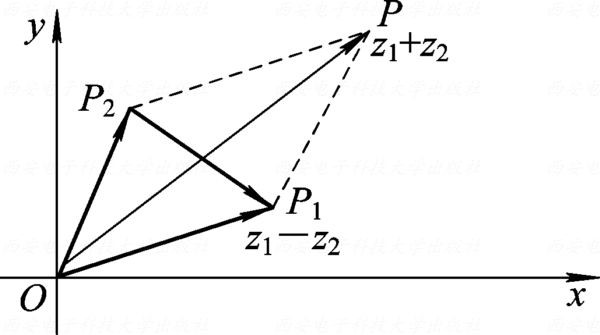
\includegraphics[height=0.6\textheight]{Figure_1_3.jpg}
		\caption{1.3}
	\end{figure}
\end{enumerate}
\end{frame}



\begin{frame}
\begin{enumerate}
	\item []
	By the parallelogram rule（平行四边形法则）, the lengths $\abs{z_1}$, $\abs{z_2}$, and $\abs{z_1-z_2}$ form the side lengths of a triangle. In particular, $\abs{z_1-z_2}$ is the length of $\overrightarrow{P_2P_1}$, that is, the distance between the points $z_1$ and $z_2$. Indeed,
	\[\resizebox*{\linewidth}{!}{$\abs{z_1-z_2}=\abs{(x_1-x_2)+i(y_1-y_2)}=\sqrt{(x_1-x_2)^2+(y_1-y_2)^2}$}\]
	which is precisely the distance formula in the plane.
\end{enumerate}
\end{frame}


\begin{frame}
\begin{enumerate}
	\item []
	The lengths $\abs{z_1}$, $\abs{z_2}$, and $\abs{z_1+z_2}$ also form the side lengths of a triangle. Therefore, the triangle inequality（三角不等式） and reverse triangle inequality（反三角不等式） give
	\[\abs{z_1+z_2}\leq\abs{z_1}+\abs{z_2},\quad\abs{z_1-z_2}\geq\abs{\abs{z_1}-\abs{z_2}}\]
	Multiplication and division are defined by
	\begin{align*}
	z_1z_2 & =(x_1x_2-y_1y_2)+i(x_1y_2+x_2y_1), \\
	\frac{z_1}{z_2}
	& =\frac{(x_1+iy_1)(x_2-iy_2)}{x_2^2+y_2^2} \\
	& =\frac{x_1x_2+y_1y_2}{x_2^2+y_2^2}+i\frac{x_2y_1-x_1y_2}{x_2^2+y_2^2}\quad(z_2\neq 0).
	\tag{1.2.2}
	\end{align*}
\end{enumerate}
\end{frame}




\begin{frame}
\begin{enumerate}
	\item []
	The multiplication and division formulas are especially transparent in trigonometric form. Let $z_1=r_1(\cos\theta_1+i\sin\theta_1)$ and $z_2=r_2(\cos\theta_2+i\sin\theta_2)$. Then\\
	\resizebox*{\linewidth}{!}{
		\begin{minipage}{1.2\linewidth}
			\begin{align*}
			z_1z_2 & =r_1r_2(\cos\theta_1+i\sin\theta_1)(\cos\theta_2+i\sin\theta_2)                                                   \\
			& =r_1r_2[(\cos\theta_1\cos\theta_2-\sin\theta_1\sin\theta_2)+i(\sin\theta_1\cos\theta_2+\cos\theta_1\sin\theta_2)] \\
			& =r_1r_2[\cos(\theta_1+\theta_2)+i\sin(\theta_1+\theta_2)]
			\tag{1.2.3}
			\end{align*}
		\end{minipage}
	}
\end{enumerate}
\end{frame}



\begin{frame}
\begin{enumerate}
	\item []
	Similarly, for $z_2\neq0$,
	\[\frac{z_1}{z_2}=\frac{r_1(\cos\theta_1+i\sin\theta_1)}{r_2(\cos\theta_2+i\sin\theta_2)}=\frac{r_1}{r_2}[\cos(\theta_1-\theta_2)+i\sin(\theta_1-\theta_2)] \tag{1.2.4}\]\\
	If $z_1=r_1e^{i\theta_1}$ and $z_2=r_2e^{i\theta_2}$, the corresponding exponential formulas are
	\[\begin{split}
	z_1z_2&=r_1e^{i\theta_1}r_2e^{i\theta_2}=r_1r_2e^{i(\theta_1+\theta_2)}\\
	\frac{z_1}{z_2}&=\frac{r_1e^{i\theta_1}}{r_2e^{i\theta_2}}=\frac{r_1}{r_2}e^{i(\theta_1-\theta_2)}\quad(r_2\neq 0)
	\end{split}
	\tag{1.2.5}\]
\end{enumerate}
\end{frame}


\begin{frame}
\begin{enumerate}
	\item []
	Consequently,
	\[\abs{z_1z_2}=\abs{z_1}\abs{z_2},\quad\abs{\frac{z_1}{z_2}}=\frac{\abs{z_1}}{\abs{z_2}} \tag{1.2.6}\]
	For principal arguments, the corresponding relations are understood modulo $2\pi$:
	\begin{equation*}
	\begin{cases}
	\arg (z_1z_2)\equiv\arg z_1+\arg z_2 \pmod{2\pi}, \\
	\arg \left(\frac{z_1}{z_2}\right)\equiv\arg z_1-\arg z_2 \pmod{2\pi}.
	\end{cases}
	\tag{1.2.7}
	\end{equation*}
\end{enumerate}
\end{frame}


\begin{frame}
\frametitle{对 $2\pi$ 求模}
对 $2\pi$ 求模，就是用 $2\pi$ 作除数求余数。余数区间必须预先规定。为了得到幅角主值，取余数区间为 $(-\pi,\pi]$。对任意 $\theta\in\mathbb R$，存在唯一的 $k\in\mathbb Z$ 和 $r\in(-\pi,\pi]$，使得
\[
\theta=2k\pi+r.
\]
此时，$r$ 是 $\theta$ 对 $2\pi$ 求模所得的余数，记作
\[
r=\theta\bmod 2\pi,\qquad -\pi<r\leq\pi.
\]
模 $2\pi$ 同余表示两个角度具有相同的余数：
\[
\theta_1\equiv\theta_2\pmod{2\pi}
\quad\Longleftrightarrow\quad
\theta_1-\theta_2=2k\pi,\quad k\in\mathbb Z.
\]
例如，$\frac{17\pi}{12}=2\pi-\frac{7\pi}{12}$，所以
\[
\frac{17\pi}{12}\bmod 2\pi=-\frac{7\pi}{12}.
\]
\end{frame}



\begin{frame}
\begin{enumerate}
	\item []
	For example, if $z_1=-1$ and $z_2=i$, then $z_1z_2=-i$, so
	\[\Arg z_1=\pi+2n\pi\quad(n\in\mathbb{Z})\]
	\[\Arg z_2=\frac{\pi}{2}+2m\pi\quad(m\in\mathbb{Z})\]
	\[\Arg z_1z_2=-\frac{\pi}{2}+2k\pi\quad(k\in\mathbb{Z})\]
\end{enumerate}
\end{frame}


\begin{frame}
\begin{enumerate}
	\item []
	Choosing arbitrary representatives of these arguments, we obtain
	\[\frac{3\pi}{2}+2(m+n)\pi=-\frac{\pi}{2}+2k\pi\]
	This equality holds exactly when $k=m+n+1$. Thus, for any chosen $m,n\in\mathbb{Z}$, an appropriate $k$ always exists, and conversely. For example, if $m=n=0$, then $k=1$; if $k=-1$, one may take $(m,n)=(0,-2)$ or $(-2,0)$.
\end{enumerate}
\end{frame}


\begin{frame}
\begin{enumerate}
	\item []
	The trigonometric and exponential forms reveal the geometric meaning of multiplication. The vector representing $z_1z_2$ is obtained from the vector representing $z_1$ by scaling（尺度变换） its length by $r_2=\abs{z_2}$ and rotating（旋转） it through an argument of $z_2$ (see Figure 1.4).
\end{enumerate}
\end{frame}


\begin{frame}
\begin{enumerate}
	\item []
	\begin{figure}
		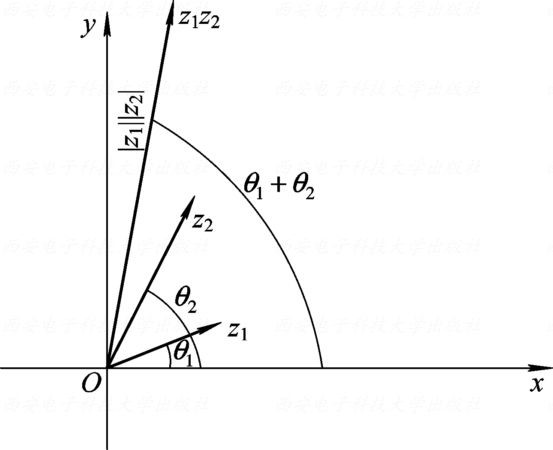
\includegraphics[height=0.8\textheight]{Figure_1_4.jpg}
		\caption{1.4}
	\end{figure}
\end{enumerate}
\end{frame}



\begin{frame}
\begin{enumerate}
	\item []
	\begin{itemize}
		\item Which expression scales the modulus of $z$ by $\sqrt{2}$ and rotates its vector counterclockwise through $\frac{\pi}{4}$?
		\[
		\mathrm{A}.z\sqrt{2}e^{-i\frac{\pi}{4}}\qquad
		\mathrm{B}.\frac{z}{\sqrt{2}}e^{-i\frac{\pi}{4}}\qquad
		\mathrm{C}.\frac{z}{\sqrt{2}}e^{i\frac{\pi}{4}}\qquad
		\mathrm{D}.z\sqrt{2}e^{i\frac{\pi}{4}}
		\]
		\item The expression $\frac{z}{1-\sqrt{3}i}$ scales the modulus of $z$ by \underline{\makebox[50pt]{}} and changes its argument by \underline{\makebox[50pt]{}}.
		\item Let $z_3=\frac{z_1}{z_2}$. Suppose $\abs{z_3}=\frac{1}{5}\abs{z_1}$ and the argument of $z_3$ is obtained by rotating the argument of $z_1$ counterclockwise through $\frac{\pi}{6}$. Find $z_2$.
	\end{itemize}
\end{enumerate}
\end{frame}



\begin{frame}
\begin{example}
	Let $z_1$ and $z_2$ be arbitrary points in the complex plane. Prove that $\abs{z_1-z_2}\geq\abs{\abs{z_1}-\abs{z_2}}$.
\end{example}
\begin{proofs}<2->
	Geometrically, the inequality states that one side of a triangle is at least the absolute difference of the other two side lengths. Algebraically, it follows from the triangle inequality $\abs{z_1+z_2}\leq\abs{z_1}+\abs{z_2}$.\\
	Because
	\[\abs{z_1}=\abs{z_1-z_2+z_2}\leq\abs{z_1-z_2}+\abs{z_2}\]
\end{proofs}
\end{frame}

\begin{frame}
\begin{proof}[\proofname\ (Cont.)]
	\[\abs{z_1}-\abs{z_2}\leq\abs{z_1-z_2} \tag{1}\]
	Because
	\[\abs{z_2}=\abs{z_2-z_1+z_1}\leq\abs{z_2-z_1}+\abs{z_1}\]
	\[\abs{z_2}-\abs{z_1}\leq\abs{z_2-z_1} \tag{2}\]
	Using inequalities (1) and (2), we have
	\[\abs{z_1-z_2}\geq\abs{\abs{z_1}-\abs{z_2}}\]
\end{proof}
\end{frame}



\begin{frame}
\begin{example}
	Two vertices\textnormal{（顶点）} of an equilateral triangle\textnormal{（等边三角形）} are $z_1=1+2i$ and $z_2=3+2i$. Find the possible third vertices.
\end{example}
\begin{solution}<2->
	As shown in Figure 1.5, fix $z_1$ and rotate the vector $z_2-z_1$ through $\frac{\pi}{3}$ or $-\frac{\pi}{3}$. The endpoint（终点） of the resulting vector is a possible third vertex $z_3$.
\end{solution}
\end{frame}


\begin{frame}
\begin{solution}[Solution\ (Cont.)]
	\begin{figure}
		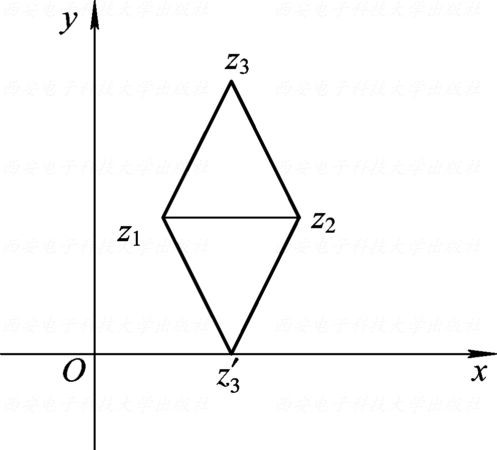
\includegraphics[height=0.6\textheight]{Figure_1_5.jpg}
		\caption{1.5}
	\end{figure}
\end{solution}
\end{frame}


\begin{frame}
\begin{enumerate}
	\item []
	As with real numbers, complex addition and multiplication satisfy the commutative, associative, and distributive laws:
	\[z_1+z_2=z_2+z_1;\ z_1z_2=z_2z_1 \tag{commutative law}\]
	\[z_1+(z_2+z_3)=(z_1+z_2)+z_3;\ z_1(z_2z_3)=(z_1z_2)z_3 \tag{associative law}\]
	\[z_1(z_2+z_3)=z_1z_2+z_1z_3 \tag{distributive law}\]
	Together with these operations, the set of complex numbers forms the complex field（复数域）, denoted by $\mathbb{C}$.
\end{enumerate}
\end{frame}



\begin{frame}
\begin{enumerate}
	\setcounter{enumi}{1}
	\item {\bf Powers and Roots of Complex Numbers}\\
	For $n\in\mathbb{N}$, the product of $n$ copies of $z$ is called the $n$-th power of $z$ and is denoted by $z^n$:
	$$z^n=\underbrace{z\cdot z\cdots z}_{n\text{ factors}}.$$
	If $z=re^{i\theta}$, then
	\[z^n=r^ne^{in\theta}=r^n(\cos n\theta+i\sin n\theta)\quad(n\in\mathbb{N})\]
	In particular, when $r=1$, de Moivre's formula（棣莫弗公式） is obtained:
	\[(\cos\theta+i\sin\theta)^n=(\cos n\theta+i\sin n\theta) \tag{1.2.8}\]
\end{enumerate}
\end{frame}


\begin{frame}
\begin{enumerate}
	\item []   For $n\in\mathbb{N}$, we have $z^n=r^n(\cos n\theta+i\sin n\theta)$. If $z\neq0$, negative integer powers are defined by $z^{-n}=1/z^n$. Thus,
	\begin{align*}
z^{-n}             & =\frac{1}{r^ne^{in\theta}}=r^{-n}e^{-in\theta} \\
                    & =r^{-n}[\cos(-n\theta)+i\sin(-n\theta)].
\end{align*}
Therefore, $z^m=r^m(\cos m\theta+i\sin m\theta)$ for every $m\in\mathbb{Z}$, provided $z\neq0$ when $m<0$.

\end{enumerate}
\end{frame}

\begin{frame}
\begin{enumerate}
	\item []
	Let $z\neq0$. If $\omega^n=z$, then $\omega$ is called an $n$-th root（$n$ 次方根） of $z$. Write $z=re^{i\theta}=r(\cos\theta+i\sin\theta)$ and $\omega=\rho e^{i\varphi}=\rho(\cos\varphi+i\sin\varphi)$. Using the power formula for the trigonometric form together with $\omega^n=z$, we obtain
	\[\rho^n(\cos n\varphi+i\sin n\varphi)=r(\cos\theta+i\sin\theta) \tag{1.2.9}\]\\
	Thus, $\rho^n=r$, $\cos n\varphi=\cos\theta$, and $\sin n\varphi=\sin\theta$. The necessary and sufficient conditions for (1.2.9) are
	\[ \rho ^n=r,\;\; n\varphi=\theta+2k\pi\quad(k\in\mathbb{Z})\]
	Therefore, $\rho=r^{1/n}$ and $\varphi=(\theta+2k\pi)/n$, where $r^{1/n}$ is the positive real $n$-th root of $r$. Hence,
	\[\omega_k=r^{1/n}\left(\cos\frac{\theta+2k\pi}{n}+i\sin\frac{\theta+2k\pi}{n}\right). \tag{1.2.10}\]

\end{enumerate}
\end{frame}


\begin{frame}
\begin{enumerate}
	\item []
	For $k=0,1,2,\ldots,n-1$, formula (1.2.10) gives $n$ distinct roots:
	\[\omega_0=r^\frac{1}{n}\left(\cos\frac{\theta}{n}+i\sin\frac{\theta}{n}\right)\]
	\[\omega_1=r^\frac{1}{n}\left(\cos\frac{\theta+2\pi}{n}+i\sin\frac{\theta+2\pi}{n}\right)\]
	\[\vdots\]
	\[\omega_{n-1}=r^\frac{1}{n}\left(\cos\frac{\theta+2(n-1)\pi}{n}+i\sin\frac{\theta+2(n-1)\pi}{n}\right)\]
	Other integer values of $k$ repeat these roots. For example,
	\[\omega_n=r^\frac{1}{n}\left(\cos\frac{\theta+2n\pi}{n}+i\sin\frac{\theta+2n\pi}{n}\right)=\omega_0\]
\end{enumerate}
\end{frame}



\begin{frame}
\begin{enumerate}
	\item []
	\begin{figure}
		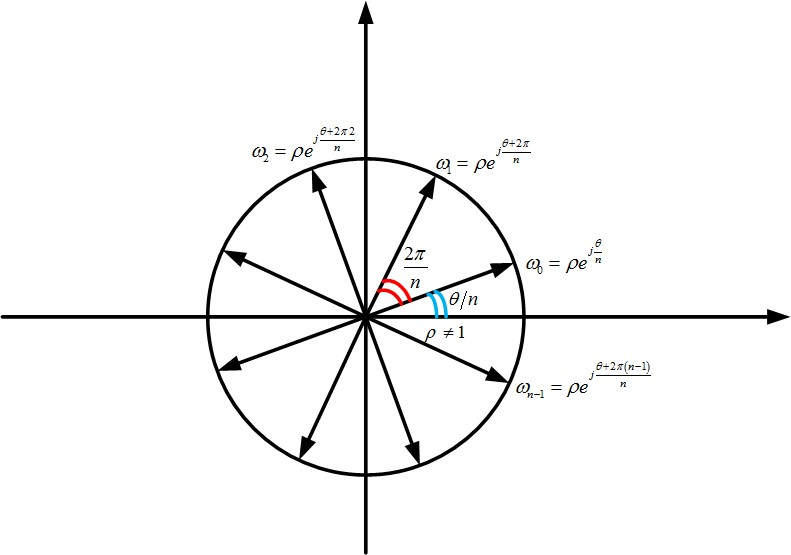
\includegraphics[height=0.85\textheight]{Figure_1_5_a.jpg}
	\end{figure}
\end{enumerate}
\end{frame}



\begin{frame}
\begin{enumerate}
	\item []
	In particular, when $z=1$, let
	\[\omega=\cos\frac{2\pi}{n}+i\sin\frac{2\pi}{n}\]
	Then the $n$-th roots of unity（单位根） are $1,\omega,\omega^2,\ldots,\omega^{n-1}$.
	
		\begin{figure}
		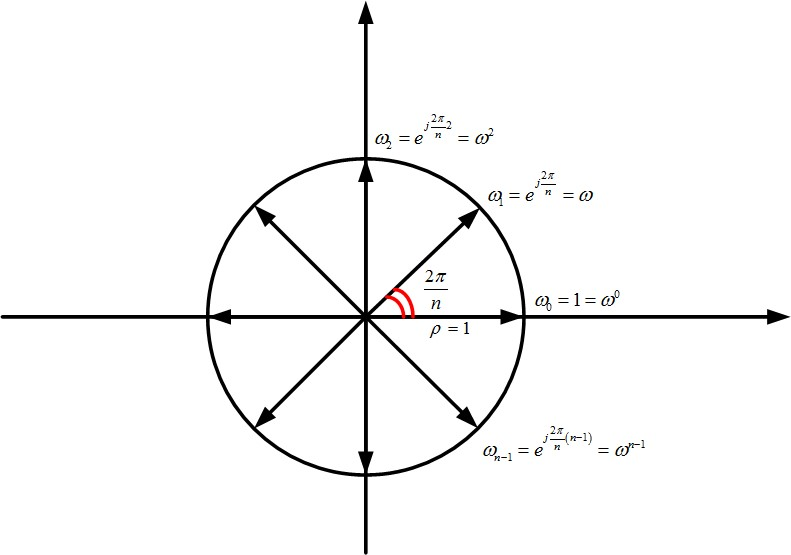
\includegraphics[height=0.5\textheight]{Figure_1_5_b.jpg}
	\end{figure}
\end{enumerate}
\end{frame}


\begin{frame}
\begin{example}
	Evaluate $\left(\frac{\sqrt{3}+i}{1-i}\right)^6$.
\end{example}
\begin{solution}<2->
	Because
	\[\sqrt{3}+i=2\left(\cos\frac{\pi}{6}+i\sin\frac{\pi}{6}\right)=2e^{\frac{\pi}{6}i}\]
	\[1-i=\sqrt{2}\left[\cos\left(-\frac{\pi}{4}\right)+i\sin\left(-\frac{\pi}{4}\right)\right]=\sqrt{2}e^{-\frac{\pi}{4}i}\]
\end{solution}
\end{frame}



\begin{frame}
\begin{solution}[Solution\ (Cont.)]
	\[\frac{\sqrt{3}+i}{1-i}=\frac{2e^{\frac{\pi}{6}i}}{\sqrt{2}e^{-\frac{\pi}{4}i}}=\sqrt{2}e^{\frac{5\pi}{12}i}\]
	Therefore,
	\[\left(\frac{\sqrt{3}+i}{1-i}\right)^6=\left(\sqrt{2}e^{\frac{5\pi}{12}i}\right)^6=8e^{\frac{5\pi}{2}i}=8\left(\cos\frac{5\pi}{2}+i\sin\frac{5\pi}{2}\right)=8i\]
\end{solution}
\end{frame}



\begin{frame}
\begin{example}
	Solve the equation $(1+z)^6=(1-z)^6$.
\end{example}
\begin{solution}<2->
	Since $z=1$ is not a solution, we may divide by $(1-z)^6$ and write
	\[\left(\frac{1+z}{1-z}\right)^6=1\]
	Let $\omega=\frac{1+z}{1-z}$, then $\omega^6=1$.
\end{solution}
\end{frame}



\begin{frame}
\begin{solution}[Solution\ (Cont.)]
	Since $1=\cos0+i\sin0$, the sixth roots of unity are
	\[\sqrt[6]{1}=\cos\frac{2k\pi}{6}+i\sin\frac{2k\pi}{6}\quad(k=0,1,2,3,4,5)\]
	then
	\[\omega_0=(\cos0+i\sin0)\]
	\[\omega_1=\left(\cos\frac{\pi}{3}+i\sin\frac{\pi}{3}\right)\]
\end{solution}
\end{frame}

\begin{frame}
\begin{solution}[Solution\ (Cont.)]
\[\omega_2=\left(\cos\frac{2\pi}{3}+i\sin\frac{2\pi}{3}\right)\]
\[\omega_3=(\cos\pi+i\sin\pi)\]
\[\omega_4=\left(\cos\frac{4\pi}{3}+i\sin\frac{4\pi}{3}\right)\]
\[\omega_5=\left(\cos\frac{5\pi}{3}+i\sin\frac{5\pi}{3}\right)\]
These six roots are the vertices of a regular hexagon（正六边形） inscribed in（内接于） the unit circle (see Figure 1.6).
\end{solution}
\end{frame}


\begin{frame}
\begin{solution}[Solution\ (Cont.)]
	\begin{figure}
		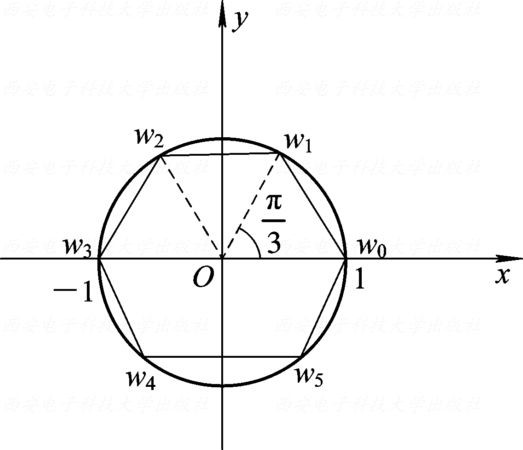
\includegraphics[height=0.6\textheight]{Figure_1_6.jpg}
		\caption{1.6}
	\end{figure}
\end{solution}
\end{frame}


\begin{frame}
\begin{solution}[Solution\ (Cont.)]
	From
	\[\omega=\frac{1+z}{1-z}\Rightarrow z=\frac{\omega-1}{\omega+1}\]
	\[z=\frac{e^{i\alpha}-1}{e^{i\alpha}+1}=\frac{\cos\alpha+i\sin\alpha-1}{\cos\alpha+i\sin\alpha+1}\]
	\[z=\frac{2\sin\frac{\alpha}{2}\left(-\sin\frac{\alpha}{2}+i\cos\frac{\alpha}{2}\right)}{2\cos\frac{\alpha}{2}\left(\cos\frac{\alpha}{2}+i\sin\frac{\alpha}{2}\right)}=\tan\frac{\alpha}{2}\frac{e^{i\left(\frac{\pi}{2}+\frac{\alpha}{2}\right)}}{e^{i\frac{\alpha}{2}}}=i\tan\frac{\alpha}{2}\]
	The value $\alpha=\pi$ corresponds to $\omega=-1$, for which $\omega+1=0$, so it yields no finite $z$. Therefore, the solutions are
	\[z=i\tan\frac{\alpha}{2},\qquad \alpha=0,\frac{\pi}{3},\frac{2\pi}{3},\frac{4\pi}{3},\frac{5\pi}{3}.\]
\end{solution}
\end{frame}



\begin{frame}
\begin{enumerate}
	\setcounter{enumi}{2}
	\item {\bf Complex Conjugate} \\
	For $z=x+iy$, its complex conjugate（共轭复数） is $\overline{z}=x-iy$. Geometrically, the points $z$ and $\overline{z}$ are symmetric（对称） about the real axis (see Figure 1.7). Hence, $\abs{z}=\abs{\overline{z}}$. If $z\neq0$ and $z$ is not on the negative real axis, then $\arg\overline{z}=-\arg z$.
	
	\begin{figure}
		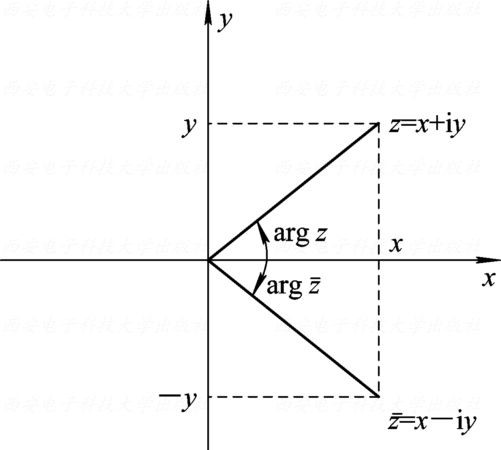
\includegraphics[height=0.5\textheight]{Figure_1_7.jpg}
		\caption{1.7}
	\end{figure}
	
\end{enumerate}
\end{frame}



\begin{frame}
Some useful properties of complex conjugation are
\begin{enumerate}


    \item  $\abs{z}=\abs{\overline{z}}$, $\arg\overline{z}\equiv-\arg z\pmod{2\pi}$ for $z\neq0$, and $\overline{\overline z}=z$;
    
    
    \item $z\overline z  = {\left[ {{\mathop{\rm Re}\nolimits} (z)} \right]^2} + {\left[ {{\mathop{\rm Im}\nolimits} (z)} \right]^2} = \left| z \right|^2$
    
	\item $z+\overline z=2\operatorname{Re}(z)$ and $z-\overline z=2i\operatorname{Im}(z)$;
	  
	  
    \item $\overline{z_1\pm z_2}=\overline z_1\pm\overline z_2$, $\overline{z_1z_2}=\overline z_1\,\overline z_2$, and $\overline{(z_1/z_2)}=\overline z_1/\overline z_2$ for $z_2\neq0$;

    \item If $P$ and $Q$ are polynomials with real coefficients and $Q(z)\neq0$, then
    $\overline{\left(\frac{P(z)}{Q(z)}\right)}
    =\frac{\overline{P(z)}}{\overline{Q(z)}}
    =\frac{P(\overline z)}{Q(\overline z)}$.
    
    
    
    
     

\end{enumerate}
\end{frame}



\begin{frame}
\begin{example}
	Let $z_1=1+2i$ and $z_2=-3-4i$. Find $\frac{z_1}{z_2}$, $\overline{\left(\frac{z_1}{z_2}\right)}$, $\operatorname{Re}\left(\frac{z_1}{z_2}\right)$, and $\operatorname{Im}\left(\frac{z_1}{z_2}\right)$.
\end{example}
\begin{solution}<2->
	\begin{align*}
	\frac{z_1}{z_2} & =\frac{1+2i}{-3-4i}=\frac{(1+2i)(-3+4i)}{(-3-4i)(-3+4i)} \\
	& =\frac{-3-8+(4-6)i}{25}=-\frac{11}{25}-\frac{2}{25}i
	\end{align*}
\end{solution}
\end{frame}



\begin{frame}
\begin{solution}[Solution\ (Cont.)]
	Therefore,
	\[\overline{\left(\frac{z_1}{z_2}\right)}=-\frac{11}{25}+\frac{2}{25}i\]\\
	and hence
	\[\operatorname{Re}\left(\frac{z_1}{z_2}\right)=-\frac{11}{25},\quad\operatorname{Im}\left(\frac{z_1}{z_2}\right)=-\frac{2}{25}\]
\end{solution}
\end{frame}


\begin{frame}
\begin{example}
	Let $a,b\in\mathbb{R}$, with $b\neq0$ and $\abs{a+ib}=1$. Prove that there exists $c\in\mathbb{R}$ such that $a+ib=\frac{c+i}{c-i}$.
\end{example}
\end{frame}



\begin{frame}
\begin{proof}
	\resizebox*{\linewidth}{!}{
		\begin{minipage}{1.2\linewidth}
			\begin{align*}
			z             & =a+ib                                                                                                 \\
			\Rightarrow z & =\frac{c+i}{c-i}                                                                                      \\
			\Rightarrow c & =\frac{z+1}{z-1}i                                                                                     \\
			\Rightarrow c & =\frac{a+ib+1}{a+ib-1}i=\frac{(a+1)+ib}{(a-1)+ib}i=\frac{[(a+1)+ib][(a-1)-ib]}{[(a-1)+ib][(a-1)-ib]}i \\
			& =\frac{(a+1)(a-1)+b^2+ib[(a-1)-(a+1)]}{(a-1)^2+b^2}i                                                  \\
			& =\frac{a^2+b^2-1-2bi}{a^2-2a+1+b^2}i                                                                  \\
			& =\frac{b}{(1-a)}\quad\left(\because a^2+b^2=1\right)
			\end{align*}
		\end{minipage}
	}
\end{proof}
\end{frame}


\begin{frame}
\begin{example}
	Let $z_1=x_1+iy_1$ and $z_2=x_2+iy_2$ be arbitrary complex numbers. Prove that\\
	\begin{enumerate}
		\item $z_1\overline{z_2}+\overline{z_1}z_2=2\operatorname{Re}(z_1\overline{z_2})$;
		\item $\abs{z_1+z_2}\leq\abs{z_1}+\abs{z_2}$.
	\end{enumerate}
\end{example}
\end{frame}




\begin{frame}
\begin{proofs}
	\begin{enumerate}
		\item $\begin{aligned}[t]
		z_1\overline{z_2}+\overline{z_1}z_2 & =(x_1+iy_1)(x_2-iy_2)+(x_1-iy_1)(x_2+iy_2) \\
		& =(x_1x_2+y_1y_2)+i(x_2y_1-x_1y_2)          \\
		& \quad+(x_1x_2+y_1y_2)+i(-x_2y_1+x_1y_2)    \\
		& =2(x_1x_2+y_1y_2)                          \\
		& =2\operatorname{Re}(z_1\overline{z_2})
		\end{aligned}$\\
		or $z_1\overline{z_2}+\overline{z_1}z_2=z_1\overline{z_2}+\overline{z_1\overline{z_2}}=2\operatorname{Re}(z_1\overline{z_2})$
	\end{enumerate}
\end{proofs}
\end{frame}



\begin{frame}
\begin{proofs}[\proofname\ (Cont.)]
	\begin{enumerate}
		\setcounter{enumi}{1}
		\item Although the triangle inequality has a geometric interpretation, we now prove it algebraically. Since
		\begin{align*}
		\abs{z_1+z_2}^2 & =(z_1+z_2)(\overline{z_1+z_2})                                             \\
		& =(z_1+z_2)(\overline{z_1}+\overline{z_2})                                \\
		& =z_1\overline{z_1}+z_2\overline{z_2}+\overline{z_1}z_2+z_1\overline{z_2} \\
		& =\abs{z_1}^2+\abs{z_2}^2+\overline{z_1}z_2+z_1\overline{z_2}
		\end{align*}
	\end{enumerate}
\end{proofs}
\end{frame}



\begin{frame}
\begin{proof}[\proofname\ (Cont.)]
	Using $z_1\overline{z_2}+\overline{z_1}z_2=2\operatorname{Re}(z_1\overline{z_2})$, we obtain
	\begin{align*}
	\abs{z_1+z_2}^2 & =\abs{z_1}^2+\abs{z_2}^2+2\operatorname{Re}(z_1\overline{z_2}) \\
	& \leq\abs{z_1}^2+\abs{z_2}^2+2\abs{z_1\overline{z_2}}           \\
	& =\abs{z_1}^2+\abs{z_2}^2+2\abs{z_1}\abs{z_2}                   \\
	& =(\abs{z_1}+\abs{z_2})^2
	\end{align*}\\
	Taking square roots on both sides completes the proof of the triangle inequality.
\end{proof}
\end{frame}



\begin{frame}
\begin{example}
	Prove that three pairwise distinct complex numbers $z_1$, $z_2$, and $z_3$ are the vertices of an equilateral triangle if and only if
	\[z_1^2+z_2^2+z_3^2=z_1z_2+z_2z_3+z_3z_1.\]
\end{example}
\begin{proofs}
	Method 1.\\
	The triangle $\triangle z_1z_2z_3$ is equilateral if and only if rotating $\overrightarrow{z_1z_2}$ through $\pm\frac{\pi}{3}$ about $z_1$ gives $\overrightarrow{z_1z_3}$. Thus, $z_3-z_1=(z_2-z_1)e^{\pm i\pi/3}$, or
\end{proofs}
\end{frame}


\begin{frame}
\begin{proof}[\proofname\ (Cont.)]
	\[\frac{z_3-z_1}{z_2-z_1}=e^{\pm i\pi/3}=\frac{1}{2}\pm i\frac{\sqrt{3}}{2},\quad\frac{z_3-z_1}{z_2-z_1}-\frac{1}{2}=\pm i\frac{\sqrt{3}}{2}.\]\\
	Squaring both sides and simplifying gives
	\[z_1^2+z_2^2+z_3^2=z_1z_2+z_2z_3+z_3z_1\]
\end{proof}
\end{frame}




\begin{frame}
\begin{proofs}
	Method 2.\\
	The equation $z_1^2+z_2^2+z_3^2=z_1z_2+z_2z_3+z_3z_1$ is equivalent to
	\[\frac{z_2-z_1}{z_3-z_1}=\frac{z_1-z_3}{z_2-z_3} \tag{1}\]
	If $z_1$, $z_2$, and $z_3$ satisfy (1), then taking absolute values after cross-multiplication gives
	\[\abs{z_3-z_1}^2=\abs{z_1-z_2}\abs{z_2-z_3} \tag{2}\]
\end{proofs}
\end{frame}

\begin{frame}
\begin{proofs}[\proofname\ (Cont.)]
\[\frac{z_2-z_1}{z_3-z_1}-1=\frac{z_1-z_3}{z_2-z_3}-1\]\\
which is equivalent to
\[\frac{z_2-z_3}{z_3-z_1}=\frac{z_1-z_2}{z_2-z_3} \tag{3}\]
Taking absolute values gives
\[\abs{z_2-z_3}^2=\abs{z_1-z_2}\abs{z_3-z_1} \tag{4}\]
\end{proofs}
\end{frame}

\begin{frame}
\begin{proofs}[\proofname\ (Cont.)]
Conversely, if $\triangle z_1z_2z_3$ is equilateral, then
\[\abs{\frac{z_2-z_1}{z_3-z_1}}=\abs{\frac{z_1-z_3}{z_2-z_3}}=1\]
\begin{equation*}
\left\{
\begin{aligned}
\arg\left(\frac{z_2-z_1}{z_3-z_1}\right)=\arg(z_2-z_1)-\arg(z_3-z_1)=\pm\frac{\pi}{3} \\
\arg\left(\frac{z_1-z_3}{z_2-z_3}\right)=\arg(z_1-z_3)-\arg(z_2-z_3)=\pm\frac{\pi}{3}
\end{aligned}
\right.
\end{equation*}
\end{proofs}
\end{frame}

\begin{frame}
\begin{proof}[\proofname\ (Cont.)]
The two arguments have the same sign, so
\[\frac{z_2-z_1}{z_3-z_1}=\frac{z_1-z_3}{z_2-z_3}\]
\end{proof}
Finally, we illustrate two geometric applications of complex numbers: (i) expressing a plane curve（平面曲线） $F(x,y)=0$ by a complex equation, and (ii) identifying the curve or region represented by a complex equation.
\end{frame}

\begin{frame}
\begin{example}
Find a complex equation for the straight line（直线） through $z_1=x_1+iy_1$ and $z_2=x_2+iy_2$.
\end{example}
\begin{solution}<2->
The line through the distinct points $(x_1,y_1)$ and $(x_2,y_2)$ has the following system of parametric equations（参数方程组）:
\[\begin{cases}
x=x_1+t(x_2-x_1) \\
y=y_1+t(y_2-y_1)
\end{cases}\quad(t\in\mathbb{R}).\]
Therefore, with $z=x+iy$, the corresponding complex parametric equation（复参数方程） is
\[z=(x_1+iy_1)+t[(x_2+iy_2)-(x_1+iy_1)]=z_1+t(z_2-z_1).\]


\end{solution}
\end{frame}

\begin{frame}
\begin{solution}[Solution\ (Cont.)]
Alternatively, write the line in general form（一般式） as $ax+by=c$, where $a,b,c\in\mathbb R$ and $(a,b)\neq(0,0)$. If $z=x+iy$, then
\[x=\frac{z+\overline{z}}{2},\quad y=\frac{z-\overline{z}}{2i}\]
Substitution gives
\[a\left(\frac{z+\overline{z}}{2}\right)+b\left(\frac{z-\overline{z}}{2i}\right)=c\]
which can be simplified as
\[(a-ib)z+(a+ib)\overline{z}=2c\]
\end{solution}
\end{frame}

\begin{frame}
\begin{example}
Describe the loci（轨迹） or regions（区域） represented by the following conditions:
\begin{enumerate}
\item $\abs{z+2i}=2$;
\item $\abs{z-i}+\abs{z+i}\leq4$;
\item $0\leq\arg(z-1)\leq\frac{\pi}{4}$ and $2\leq\operatorname{Re}z\leq3$.
\end{enumerate}
\end{example}
\begin{solution}<2->
\begin{enumerate}
\item The equation $\abs{z+2i}=2$ describes all points at distance $2$ from $-2i$. Hence, it represents the circle（圆） centered at $-2i$ with radius（半径） $2$ (see Figure 1.8(a)).
\end{enumerate}
\end{solution}
\end{frame}

\begin{frame}
\begin{solution}[Solution\ (Cont.)]
\begin{figure}
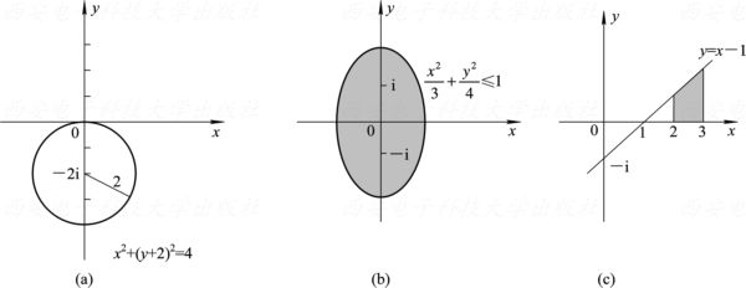
\includegraphics[width=\linewidth]{Figure_1_8.jpg}
\caption{1.8}
\end{figure}
\end{solution}
\end{frame}



\begin{frame}
\begin{enumerate}
	\setcounter{enumi}{3}
	\item {\bf The Riemann Sphere and the Point at Infinity}\\
	Consider a sphere（球面） tangent to（相切于） the complex plane at the origin $O$. Let the point of tangency（切点） be the south pole（南极） $S$, and let the perpendicular diameter（垂直直径） through $S$ meet the sphere again at the north pole（北极） $N$ (see Figure 1.9). For each point $z$ in the complex plane, the line through $N$ and $z$ meets the sphere at exactly one additional point $P$. Conversely, every point $P\neq N$ determines exactly one point $z$ in the plane. This correspondence is called stereographic projection（球极投影）, and the sphere is called the Riemann sphere（复球面）.
\end{enumerate}
\end{frame}

\begin{frame}
\begin{figure}
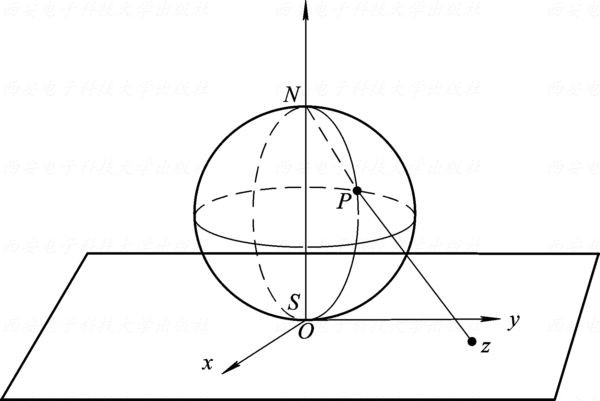
\includegraphics[height=0.8\textheight]{Figure_1_9.jpg}
\caption{1.9}
\end{figure}
\end{frame}

\begin{frame}
\begin{enumerate}
\item []
The complex plane together with the point at infinity（无穷远点） $\infty$ is called the extended complex plane（扩充复平面）. Under stereographic projection, finite points correspond to points on the sphere other than $N$, while $\infty$ corresponds to $N$. Thus, the Riemann sphere is a geometric model of the extended complex plane.
\end{enumerate}
\end{frame}

\begin{frame}
\begin{enumerate}
\item []
There is only one point at infinity in the extended complex plane; it is not separated into $+\infty$ and $-\infty$ as on the extended real line. The point $\infty$ is not an ordinary complex number, so its real part, imaginary part, and argument are undefined. With the extended-modulus convention, one writes $\abs{\infty}=+\infty$.
\end{enumerate}
\end{frame}

\begin{frame}
\begin{enumerate}
\item []
For a finite complex number $a$, arithmetic involving $\infty$ is only partially defined:
\begin{itemize}
\item Addition and subtraction: $a+\infty=\infty+a=\infty$ and $a-\infty=\infty-a=\infty$;
\item Multiplication: $a\cdot\infty=\infty\cdot a=\infty$ for $a\neq0$;
\item Division: $a/\infty=0$ for finite $a$, while $\infty/a=\infty$ and $a/0=\infty$ for finite $a\neq0$;
\item The forms $\infty-\infty$, $0\cdot\infty$, $\infty/\infty$, and $0/0$ are undefined.
\end{itemize}
\end{enumerate}
\end{frame}

\section{Regions in the Complex Plane}
\begin{frame}
	\frametitle{Outline}
	\tableofcontents[currentsection] 
\end{frame}

\begin{frame}
	\begin{enumerate}
		\item Concepts of Point Sets in the Complex Plane\\
		We begin with a point $z_0$ in the complex plane.
	\end{enumerate}
	\begin{definition}
		For $\delta>0$, the open disk centered at $z_0$ with radius $\delta$ is
		\[N_\delta(z_0)=\{z:\abs{z-z_0}<\delta\}.\]
		It is called the $\delta$-neighborhood（$\delta$ 邻域） of $z_0$ (see Figure 1.10). The set
		\[N_\delta^*(z_0)=\{z:0<\abs{z-z_0}<\delta\}\]
		is called the deleted $\delta$-neighborhood（$\delta$ 去心邻域） of $z_0$.
	\end{definition}
\end{frame}

\begin{frame}
	\begin{definition}[Cont.]
		\begin{figure}
			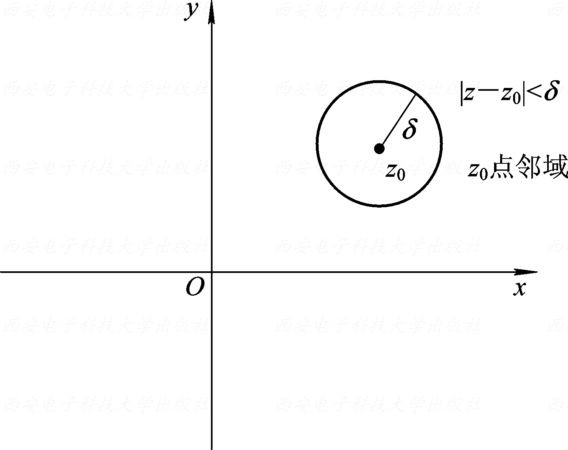
\includegraphics[height=0.6\textheight]{Figure_1_10.jpg}
			\caption{1.10}
		\end{figure}
	\end{definition}
\end{frame}


\begin{frame}
\begin{definition}
	Let $G$ be a point set（点集） in the complex plane.
	\begin{itemize}
	\item A point $z_0\in G$ is an interior point（内点） of $G$ if some neighborhood of $z_0$ is contained in $G$.
	
	\item The set $G$ is an open set（开集） if every point of $G$ is an interior point.
	
	\item A point $z_0\in\mathbb C$ is a boundary point（边界点） of $G$ if every neighborhood of $z_0$ contains both points of $G$ and points not in $G$.
	
	\item The set of all boundary points is the boundary（边界） of $G$, denoted by $\partial G$. It may consist of several curves together with isolated points (see Figure 1.11).
    \end{itemize}
\end{definition}
\end{frame}



\begin{frame}
\begin{definition}[Cont.]
	\begin{figure}
		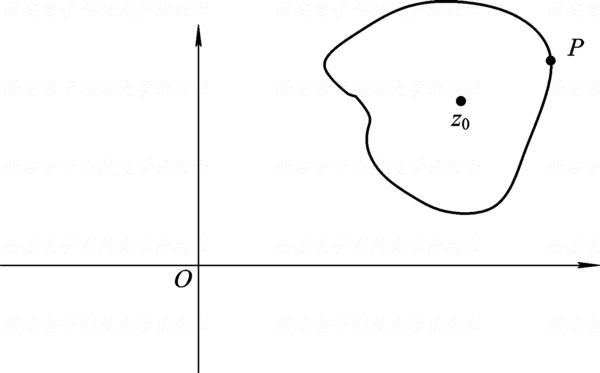
\includegraphics[height=0.6\textheight]{Figure_1_11.jpg}
		\caption{1.11}
	\end{figure}
\end{definition}
\end{frame}



\begin{frame}
\begin{definition}
	A point $z_0\in G$ is an isolated point（孤立点） of $G$ if there is a $\delta>0$ such that $N_\delta^*(z_0)\cap G=\varnothing$.
\end{definition}
\begin{definition}
	A set $G$ is bounded（有界） if there is an $R>0$ such that $\abs z<R$ for every $z\in G$. Otherwise, $G$ is unbounded（无界）.
\end{definition}
\end{frame}



\begin{frame}
\begin{definition}
	In the extended complex plane, a neighborhood of infinity（无穷远点邻域） has the form
	\[N_R(\infty)=\{z:\abs z>R\}\cup\{\infty\},\qquad R>0.\]
	Removing $\infty$ gives the deleted neighborhood of infinity（无穷远点去心邻域） $N_R^*(\infty)=\{z:\abs z>R\}$.
\end{definition}
\end{frame}




\begin{frame}
\begin{enumerate}
	\setcounter{enumi}{1}
	\item {\bf The Concept of Domains}
\end{enumerate}



\begin{definition}
	A nonempty subset $D$ of the complex plane is a domain（区域） if it satisfies both conditions:
	\begin{itemize}
		\item $D$ is an open set;
		\item $D$ is connected（连通）: any two points in $D$ can be joined by a polygonal path（折线路径） lying entirely in $D$.
	\end{itemize}
	Thus, a domain is an open connected set. Its closure $\overline D=D\cup\partial D$ is sometimes called the associated closed domain（闭区域）.
\end{definition}
\end{frame}




\begin{frame}
\begin{enumerate}
	\item []
	The following sets are domains:
	\begin{enumerate}[(1)]
		\item The open disk（开圆盘） centered at the origin: $\abs z<R$;
		\item The annulus（圆环域） in Figure 1.12(a): $r<\abs z<R$;
		\item The horizontal strip（水平带状域） in Figure 1.12(b): $y_1<\operatorname{Im}z<y_2$;
		
		\item The upper and lower half-planes（半平面）: $\operatorname{Im}z>0$ and $\operatorname{Im}z<0$;
		
		\item The left and right half-planes: $\operatorname{Re}z<0$ and $\operatorname{Re}z>0$;
		
		\item The sector（角域） in Figure 1.12(c): $0<\arg z<\varphi$, where $0<\varphi\leq\pi$.
	\end{enumerate}
\end{enumerate}
\end{frame}


\begin{frame}
\begin{enumerate}
	\item []
	\begin{figure}
		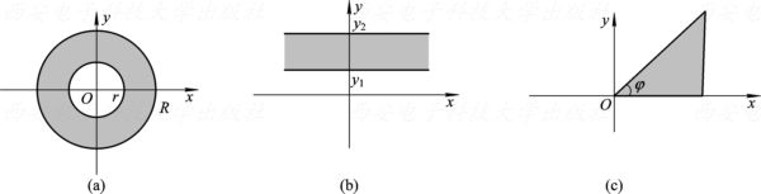
\includegraphics[width=\linewidth]{Figure_1_12.jpg}
		\caption{1.12}
	\end{figure}
\end{enumerate}
\end{frame}


\begin{frame}
\begin{enumerate}
	\setcounter{enumi}{2}
	\item {\bf Jordan Curve}
\end{enumerate}
\begin{definition}
	Let $x(t)$ and $y(t)$ be continuous real-valued functions on $[a,b]$. The parametric equations
	\[x=x(t),\qquad y=y(t)\quad(a\leq t\leq b)\]
	define a continuous curve（连续曲线） in the plane. Equivalently, the curve has the complex parametrization
	\[z=z(t)=x(t)+iy(t)\quad(a\leq t\leq b).\]
	The points $z(a)$ and $z(b)$ are its initial point（起点） and terminal point（终点）, respectively.
\end{definition}
\end{frame}



\begin{frame}
\begin{definition}[Cont.]
\begin{itemize}
	\item If $t_1\neq t_2$ and $z(t_1)=z(t_2)$, the common point is called a self-intersection point（自交点） of $C$. For a closed curve, the starting point and the endpoint coincide, but this is not considered a self-intersection.
	
	\item A continuous curve with no self-intersection is called a simple curve（简单曲线）.
	
	\item If $z(a)=z(b)$ and there are no other self-intersections, then $C$ is a simple closed curve, also called a Jordan curve（若尔当曲线）.
\end{itemize}
\end{definition}


\begin{enumerate}
	\item []
	For example, the circle $\abs z=R$ is a Jordan curve. It separates the complex plane into two disjoint domains: the bounded interior $\abs z<R$ and the unbounded exterior $\abs z>R$. Their common boundary is $\abs z=R$.
\end{enumerate}

\end{frame}


\begin{frame}
\begin{definition}
	Let $C:z=z(t)=x(t)+iy(t)$, $\alpha\leq t\leq\beta$, be a simple or simple closed curve. If $x'(t)$ and $y'(t)$ are continuous and
	\[[x'(t)]^2+[y'(t)]^2\neq0\]
	for every $t$, then $C$ is a smooth curve（光滑曲线）. A curve made of finitely many smooth arcs is a piecewise smooth curve（分段光滑曲线）.
\end{definition}
\end{frame}


\begin{frame}
\begin{enumerate}
	\setcounter{enumi}{3}
	\item {\bf Simply and Multiply Connected Domains}\\
	Simple closed curves distinguish simply connected domains from multiply connected domains.
\end{enumerate}
\begin{definition}
	A domain $D$ is simply connected（单连通） if the interior of every simple closed curve contained in $D$ also lies in $D$. Otherwise, $D$ is multiply connected（多连通）.
\end{definition}

\begin{enumerate}
	\item []
	For example, the disk $\abs z<R$ is simply connected, whereas the punctured disk（穿孔圆盘） $0<\abs z<R$ is multiply connected because it has a hole at $z=0$. More generally, a domain containing a hole is multiply connected.
\end{enumerate}
\end{frame}


\begin{frame}
\begin{example}
	Describe the point set $P=\{z=r(\cos\theta+i\sin\theta)\}$ for which
	\[2\cos\theta<r<4\cos\theta\left(-\frac{\pi}{2}<\theta<\frac{\pi}{2}\right).\]
	Is this set a domain? If so, is it bounded or unbounded, and is it simply or multiply connected?
\end{example}
\end{frame}


\begin{frame}
\begin{solution}
	Write
	\[z=x+iy=r(\cos\theta+i\sin\theta)\]
	Then
	\[r=\sqrt{x^2+y^2}\]
	\[\cos\theta=\frac{x}{\sqrt{x^2+y^2}}\]
\end{solution}
\end{frame}

\begin{frame}
\begin{solution}[Solution.\ (Cont.)]
	Because $2\cos\theta<r<4\cos\theta$,
	\[2r\cos\theta<r^2<4r\cos\theta,\quad2x<x^2+y^2<4x\]
	The first inequality gives $(x-1)^2+y^2>1$, and the second gives $(x-2)^2+y^2<4$. Thus, the point set is the shaded region in Figure 1.13:
	\[\begin{cases}
	(x-1)^2+y^2>1 \\
	(x-2)^2+y^2<4
	\end{cases}\]
	Therefore, the set is a bounded, simply connected domain.
\end{solution}
\end{frame}




\begin{frame}
\begin{solution}[Solution.\ (Cont.)]
	\begin{figure}
		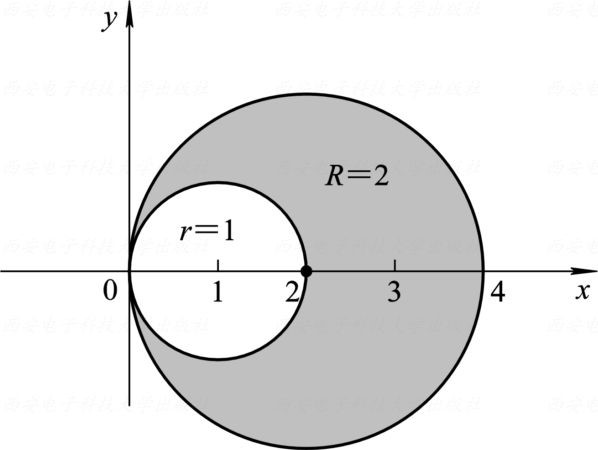
\includegraphics[height=0.6\textheight]{Figure_1_13.jpg}
		\caption{1.13}
	\end{figure}
\end{solution}
\end{frame}


\begin{frame}
\begin{example}
	Does the set of points satisfying $\operatorname{Im}z>1$ and $\abs z<2$ form a domain? If so, is it bounded, and is it simply or multiply connected?
\end{example}
\begin{solution}<2->
	Let $z=x+iy$. The conditions become $y>1$ and $x^2+y^2<4$. The shaded set in Figure 1.14 is a bounded, simply connected domain.
\end{solution}
\end{frame}


\begin{frame}
\begin{solution}[Solution.\ (Cont.)]
	\begin{figure}
		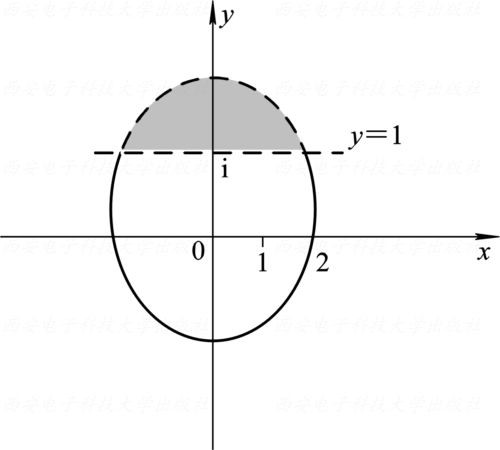
\includegraphics[height=0.6\textheight]{Figure_1_14.jpg}
		\caption{1.14}
	\end{figure}
\end{solution}
\end{frame}



\section{Complex Functions}
\begin{frame}
	\frametitle{Outline}
	\tableofcontents[currentsection] 
\end{frame}





\begin{frame}
\begin{enumerate}
	\item {\bf Definition of a Complex Function}
\end{enumerate}
\begin{definition}
	Let $G\subseteq\mathbb C$. A complex function（复变函数） $f$ on $G$ is a rule that assigns a unique complex number $w$ to each $z\in G$. We write
	\[w=f(z),\qquad z\in G.\]
	The set $G$ is the domain of definition（定义域） of $f$.
\end{definition}
\end{frame}




\begin{frame}
\begin{definition}[Cont.]
	A function assigns exactly one value $w$ to each $z$ and is therefore single-valued（单值）. A rule that assigns two or more values to some $z$ is more precisely a multiple-valued correspondence（多值对应）, although it is often called a multiple-valued function. The set
	\[f(G)=\{f(z):z\in G\}\]
	is the range（值域） of $f$.
\end{definition}
\end{frame}


\begin{frame}
\begin{definition}[Cont.]
	Writing $z=x+iy$ and $w=u+iv$ identifies each complex number with two real coordinates. Hence, a complex function $w=f(z)$ can be written as
	\[f(x+iy)=u(x,y)+iv(x,y),\]
	where $u$ and $v$ are real-valued functions（实值函数） of the two real variables $x$ and $y$.
\end{definition}
\end{frame}



\begin{frame}
\begin{definition}[Cont.]
Let $w=f(z)$, with $z=x+iy$ and $w=u+iv$. Then

\[f(z)=w=u+iv,\qquad
f(x+iy)=u(x,y)+iv(x,y).\]

\end{definition}
\end{frame}



\begin{frame}
\begin{enumerate}
	\item []
	For example, consider $w=z^2$. Let $z=x+iy$ and $w=u+iv$. Then
	\[u+iv=(x+iy)^2=x^2-y^2+2xyi,\]
	so $w=z^2$ corresponds to the two real-valued functions
	\[u(x,y)=x^2-y^2,\qquad v(x,y)=2xy.\]
\end{enumerate}
\end{frame}


\begin{frame}
\begin{enumerate}
	\setcounter{enumi}{1}
	\item {\bf The Concept of Mapping}\\
	Under the mapping（映射） $w=f(z)$, the point $w$ is the image（像） of $z$, and $z$ is a preimage（原像） of $w$. We call the domain plane the $z$-plane and the image plane the $w$-plane (see Figure 1.15).
\end{enumerate}

\begin{figure}
	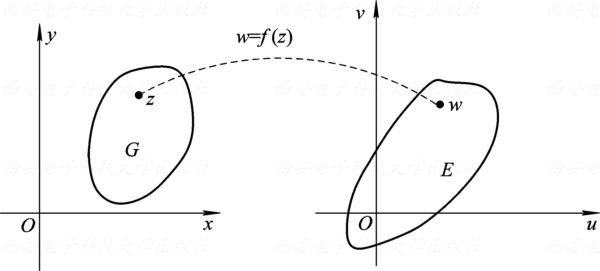
\includegraphics[width=0.7\linewidth]{Figure_1_15.jpg}
	\caption{1.15}
\end{figure}

\end{frame}



\begin{frame}
\begin{enumerate}
	\item []
	For example, $w=\overline z$ maps $z=x+iy$ in the $z$-plane to $w=x-iy$ in the $w$-plane. Thus, $z_1=1+4i$ maps to $w_1=1-4i$, $z_2=1-3i$ maps to $w_2=1+3i$, and $\triangle ABC$ maps to $\triangle A'B'C'$ (see Figure 1.16).
\end{enumerate}

\begin{figure}
	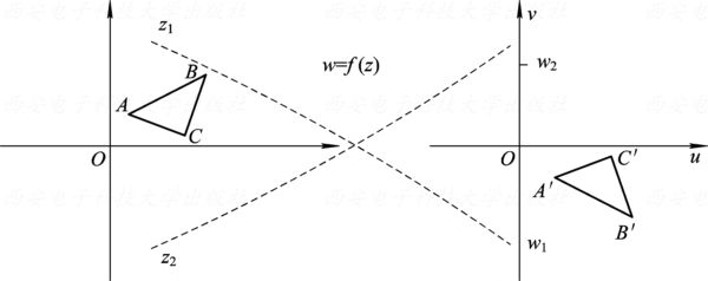
\includegraphics[width=0.8\linewidth]{Figure_1_16.jpg}
	\caption{1.16}
\end{figure}

\end{frame}


\begin{frame}
\begin{example}
	Investigate the mapping properties of the function $w=z^2$.
\end{example}
\begin{solution}<2->
	\begin{enumerate}
		\item If $z=re^{i\theta}$ and $w=\rho e^{i\varphi}$, then $w=z^2$ gives
		$$\begin{cases}
		\rho=r^2 \\
		\varphi\equiv2\theta\pmod{2\pi}
		\end{cases}$$ 
		This yields the following mapping properties:
	\end{enumerate}
\end{solution}
\end{frame}


\begin{frame}
\begin{solution}[Solution.\ (Cont.)]
	\begin{enumerate}
		\item []
		\begin{enumerate}[(1)]
			\item The ray（射线） $\{re^{i\theta_0}:r\geq0\}$ in the $z$-plane maps to $\{\rho e^{i2\theta_0}:\rho\geq0\}$ in the $w$-plane, as shown in Figure 1.17(a), (b).
			\item For $0\leq\alpha\leq\pi/2$, the sector $D=\{re^{i\theta}:r\geq0,\ 0\leq\theta\leq\alpha\}$ maps to $G=\{\rho e^{i\varphi}:\rho\geq0,\ 0\leq\varphi\leq2\alpha\}$, as shown in Figure 1.17(c), (d).
		\end{enumerate}
	\end{enumerate}
\begin{figure}
	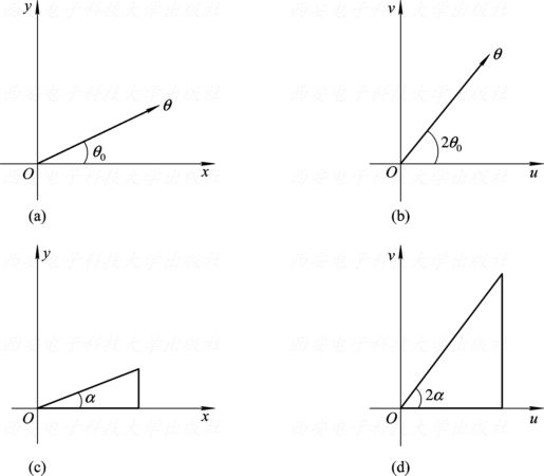
\includegraphics[height=0.37\textheight]{Figure_1_17.jpg}
	\caption{1.17}
\end{figure}
\end{solution}
\end{frame}


\begin{frame}
\begin{solution}[Solution.\ (Cont.)]
	\begin{enumerate}
		\setcounter{enumi}{1}
		\item If $z=x+iy$ and $w=u+iv$, then $w=z^2$ gives
		$$\left\{\begin{array}{ll}u=x^2-y^2\\ v=2xy.\end{array}\right.$$
		Therefore:
		\begin{enumerate}[(1)]
			\item For $c_1\neq0$, the curves $x^2-y^2=c_1$ are rectangular hyperbolas（等轴双曲线） with asymptotes（渐近线） $y=\pm x$; they map to the vertical lines $u=c_1$. For $c_2\neq0$, the curves $2xy=c_2$ have the coordinate axes as asymptotes; they map to the horizontal lines $v=c_2$ (see Figure 1.18).
		\end{enumerate}
	\end{enumerate}
\end{solution}
\end{frame}


\begin{frame}
\begin{solution}[Solution.\ (Cont.)]
	\begin{enumerate}
		\item []
		\begin{enumerate}
			\item []
			\begin{figure}
				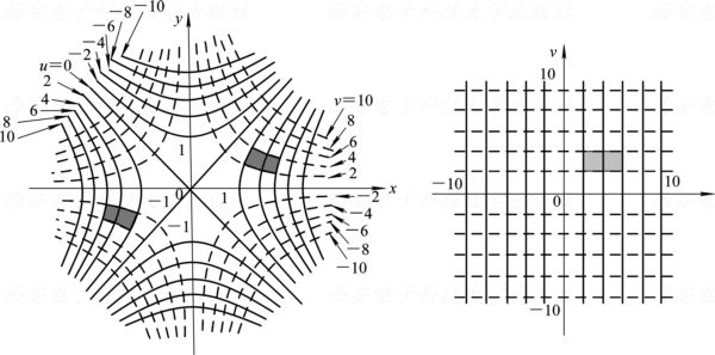
\includegraphics[width=\linewidth]{Figure_1_18.jpg}
				\caption{1.18}
			\end{figure}
		\end{enumerate}
	\end{enumerate}
\end{solution}
\end{frame}




\begin{frame}
\begin{solution}[Solution.\ (Cont.)]
	\begin{enumerate}
		\item []
		\begin{enumerate}
			\setcounter{enumii}{1}
			\item We next determine the images of the two families of lines $x=c_1$ and $y=c_2$ under $w=z^2$.\\
			For $x=c_1$, a line parallel to the imaginary axis in the $z$-plane, we have
			\begin{equation*}
			\left\{
			\begin{aligned}
			u&=c_1^2-y^2 \\
			v&=2c_1y
			\end{aligned}
			\right.
			\quad(-\infty<y<\infty).
			\end{equation*}
			Eliminating $y$ gives
			\[v^2=4c_1^2(c_1^2-u)\]
		\end{enumerate}
	\end{enumerate}
\end{solution}
\end{frame}



\begin{frame}
\begin{solution}[Solution.\ (Cont.)]
	\begin{enumerate}
		\item []
		\begin{enumerate}
			\item []
			These are parabolas（抛物线） in the $w$-plane, shown as dashed curves in Figure 1.19(b).\\
			When $c_1=0$, the line is the imaginary axis $x=0$, and its image satisfies
			\begin{equation*}
			\left\{
			\begin{aligned}
			u & =-y^2 \\
			v & =0
			\end{aligned}
			\right.
			\Rightarrow 
			\left\{
			\begin{aligned}
			u\leq 0 \\
			v=0
			\end{aligned}
			\right.
			\end{equation*}
			Thus, $w=z^2$ maps the imaginary axis in the $z$-plane onto the nonpositive real axis in the $w$-plane.
		\end{enumerate}
	\end{enumerate}
\end{solution}
\end{frame}



\begin{frame}
\begin{solution}[Solution.\ (Cont.)]
	\begin{enumerate}
		\item []
		\begin{enumerate}
			\item []
			\begin{figure}
				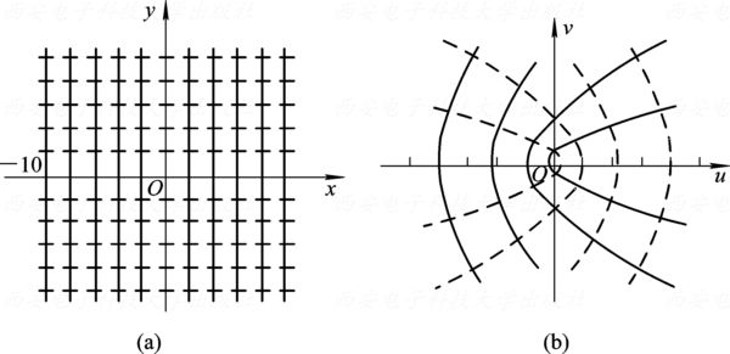
\includegraphics[width=\linewidth]{Figure_1_19.jpg}
				\caption{1.19}
			\end{figure}
		\end{enumerate}
	\end{enumerate}
\end{solution}
\end{frame}



\begin{frame}
\begin{solution}[Solution.\ (Cont.)]
	\begin{enumerate}
		\item []
		\begin{enumerate}
			\item []
			Similarly, the line $y=c_2$, shown dotted in Figure 1.19(a), maps under $w=z^2$ to the parabola
			\[v^2=4c_2^2\left(u+c_2^2\right)\]
			
			These are the solid curves in Figure 1.19(b). When $c_2=0$, the line is the real axis $y=0$, and its image satisfies
			\begin{equation*}
			\left\{
			\begin{aligned}
			u & =x^2 \\
			v & =0
			\end{aligned}
			\right.
			\text{that is}
			\left\{
			\begin{aligned}
			u\geq 0 \\
			v=0
			\end{aligned}
			\right.
			\end{equation*}
			Thus, the real axis in the $z$-plane maps onto the nonnegative real axis in the $w$-plane.
		\end{enumerate}
	\end{enumerate}
\end{solution}
\end{frame}



\begin{frame}
\begin{example}
	Under the mapping $w=z+\frac{1}{z}$, find the image of the circle $\abs z=2$.
\end{example}
\begin{solution}<2->
	Let $z=x+iy$ and $w=u+iv$. Then
	\[u+iv=x+iy+\frac{x-iy}{x^2+y^2},\]
	so
	\begin{equation*}
	\left\{
	\begin{aligned}
	u & =x+\frac{x}{x^2+y^2} \\
	v & =y-\frac{y}{x^2+y^2}
	\end{aligned}
	\right.
	\tag{1}
	\end{equation*}
\end{solution}
\end{frame}


\begin{frame}
\begin{solution}[Solution.\ (Cont.)]
	Parametrize $\abs z=2$ by $x=2\cos\theta$ and $y=2\sin\theta$, where $0\leq\theta\leq2\pi$. Substitution into (1) gives
	\[u=\frac52\cos\theta,\qquad v=\frac32\sin\theta.\]
	Therefore, the image is the ellipse（椭圆）
	\[\frac{u^2}{(5/2)^2}+\frac{v^2}{(3/2)^2}=1\]
	in the $w$-plane.
\end{solution}
\end{frame}


\section{Limits and Continuity of Complex Functions}
\begin{frame}
	\frametitle{Outline}
	\tableofcontents[currentsection] 
\end{frame}



\begin{frame}
\begin{enumerate}
	\item {\bf Limits of Complex Functions}
\end{enumerate}
\begin{definition}
	Suppose $f$ is defined in a deleted neighborhood of $z_0$. A complex number $A$ is the limit（极限） of $f(z)$ as $z\to z_0$ if, for every $\varepsilon>0$, there exists a $\delta>0$ such that
	\[0<\abs{z-z_0}<\delta\quad\Longrightarrow\quad\abs{f(z)-A}<\varepsilon.\]
	We write
	\[\lim_{z\to z_0}f(z)=A\]
	or $f(z)\to A$ as $z\to z_0$ (see Figure 1.20).
	
	The same value $A$ must be obtained along every path by which $z$ approaches $z_0$.
\end{definition}
\end{frame}


\begin{frame}
\begin{definition}[Cont.]
	\begin{figure}
		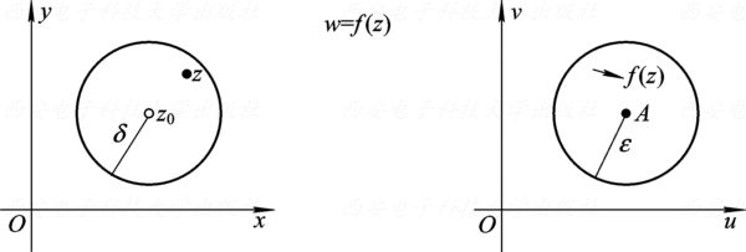
\includegraphics[width=\linewidth]{Figure_1_20.jpg}
		\caption{1.20}
	\end{figure}
\end{definition}
\end{frame}


\begin{frame}
\begin{theorem}
	Let $f(z)=u(x,y)+iv(x,y)$, $A=a+ib$, and $z_0=x_0+iy_0$. Then
	\[\lim_{z\to z_0}f(z)=A\]
	if and only if
	\[\lim_{\substack{x\to x_0\\ y\to y_0}}u(x,y)=a,\quad\lim_{\substack{x\to x_0\\ y\to y_0}}v(x,y)=b.\]
\end{theorem}
\end{frame}

\begin{frame}
\begin{proofs}
	Assume $\lim_{z\to z_0}f(z)=A$. For every $\varepsilon>0$, there is a $\delta>0$ such that
	\[0<\sqrt{(x-x_0)^2+(y-y_0)^2}<\delta\]
	implies
	\[\abs{(u+iv)-(a+ib)}<\varepsilon\]
	that is,
	\[\abs{(u-a)+i(v-b)}<\varepsilon.\]
\end{proofs}
\end{frame}



\begin{frame}
\begin{proofs}[\proofname\ (Cont.)]
	Since the absolute values of the real and imaginary parts do not exceed the modulus,
	\[\abs{u-a}<\varepsilon,\quad\abs{v-b}<\varepsilon\]
	whenever $0<\sqrt{(x-x_0)^2+(y-y_0)^2}<\delta$. Therefore,
	\[\lim_{\substack{x\to x_0\\ y\to y_0}}u(x,y)=a,\quad\lim_{\substack{x\to x_0\\ y\to y_0}}v(x,y)=b\]
\end{proofs}
\end{frame}


\begin{frame}
\begin{proofs}[\proofname\ (Cont.)]
	Conversely, assume the two real limits hold. Given $\varepsilon>0$, choose $\delta_1,\delta_2>0$ such that
	\[\abs{u-a}<\frac{\varepsilon}{2}\quad\text{if }0<\abs{z-z_0}<\delta_1,\]
	\[\abs{v-b}<\frac{\varepsilon}{2}\quad\text{if }0<\abs{z-z_0}<\delta_2.\]
	Let $\delta=\min\{\delta_1,\delta_2\}$. Then
	\[\abs{f(z)-A}=\abs{(u-a)+i(v-b)}\leq\abs{u-a}+\abs{v-b}\]
	so $0<\abs{z-z_0}<\delta$ implies $\abs{f(z)-A}<\varepsilon$. Hence, $\lim_{z\to z_0}f(z)=A$.
\end{proofs}
\end{frame}


\begin{frame}
\begin{property}
	If $\lim_{z\to z_0}f(z)$ exists, it is unique.
\end{property}
\begin{property}
	If $\lim_{z\to z_0}f(z)$ exists, then $f$ is bounded in some deleted neighborhood of $z_0$.
\end{property}
\end{frame}


\begin{frame}
\begin{theorem}
	Suppose $f$ and $g$ satisfy
	\[\lim_{z\to z_0}f(z)=A,\quad\lim_{z\to z_0}g(z)=B.\]
	Then
	\begin{enumerate}
		\item $\lim_{z\to z_0}[f(z)\pm g(z)]=A\pm B$;
		\item $\lim_{z\to z_0}[f(z)g(z)]=AB$;
		\item $\lim_{z\to z_0}\frac{f(z)}{g(z)}=\frac{A}{B}\quad(B\neq 0)$.
	\end{enumerate}
\end{theorem}
\end{frame}


\begin{frame}
\begin{example}
	Show that $f(z)=\frac{\operatorname{Re}z}{\abs z}$ has no limit as $z\to0$.
\end{example}
\begin{proofs}
	For $z=x+iy$,
	\[u(x,y)=\frac{x}{\sqrt{x^2+y^2}},\quad v(x,y)=0\]
\end{proofs}
\end{frame}


\begin{frame}
\begin{proof}[\proofname\ (Cont.)]
	Along the positive real axis, let $z=x$ with $x\to0^+$. Then
	\[f(x)=\frac{x}{\abs x}=1.\]
	Along the imaginary axis, let $z=iy$ with $y\to0$. Then
	\[f(iy)=0.\]
	The two path limits are different, so $\lim_{z\to0}f(z)$ does not exist.
\end{proof}
\end{frame}


\begin{frame}
\begin{example}
	Find the following limits:
	\begin{enumerate}
		\item $\lim_{z\to i}\frac{z-i}{z\left(1+z^2\right)}$
		\item $\lim_{z\to 1}\frac{z\overline{z}+2z-\overline{z}-2}{z^2-1}$
	\end{enumerate}
\end{example}
\end{frame}


\begin{frame}
\begin{solution}
	\begin{enumerate}
		\item \[\lim_{z\to i}\frac{z-i}{z\left(1+z^2\right)}=\lim_{z\to i}\frac{z-i}{z(z-i)(z+i)}=\lim_{z\to i}\frac{1}{z(z+i)}=-\frac{1}{2}\]
		\item \[\lim_{z\to 1}\frac{z\overline{z}+2z-\overline{z}-2}{z^2-1}=\lim_{z\to 1}\frac{(\overline{z}+2)(z-1)}{(z+1)(z-1)}=\lim_{z\to 1}\frac{(\overline{z}+2)}{(z+1)}=\frac{3}{2}\]
	\end{enumerate}
\end{solution}
\end{frame}



\begin{frame}
\begin{enumerate}
	\setcounter{enumi}{1}
	\item {\bf Continuity（连续性） of Complex Functions}
\end{enumerate}
\begin{definition}
	Let $f$ be defined near $z_0$. It is continuous at $z_0$ if
	\[\lim_{z\to z_0}f(z)=f(z_0).\]
	Continuity at $\infty$ is defined analogously using neighborhoods of infinity. If $f$ is continuous at every point of a domain $D$, then $f$ is continuous on $D$.
\end{definition}
\end{frame}


\begin{frame}
\begin{theorem}
	The complex function $f(z)=u(x,y)+iv(x,y)$ is continuous at $z_0=x_0+iy_0$ if and only if both $u$ and $v$ are continuous at $(x_0,y_0)$, that is,
	\[\lim_{\substack{x\to x_0\\ y\to y_0}}u(x,y)=u(x_0,y_0)\]
	\[\lim_{\substack{x\to x_0\\ y\to y_0}}v(x,y)=v(x_0,y_0)\]
\end{theorem}
\end{frame}


\begin{frame}
\begin{theorem}
	\begin{enumerate}
		\item Sums, differences, and products of functions continuous at $z_0$ are continuous at $z_0$. Their quotient is also continuous there if the denominator is nonzero at $z_0$.
		\item If $g$ is continuous at $z_0$ and $f$ is continuous at $g(z_0)$, then the composite function（复合函数） $f\circ g$ is continuous at $z_0$.
	\end{enumerate}
\end{theorem}
\end{frame}


\begin{frame}
\begin{example}
	Prove that $f(z)$ is not continuous at the origin, where
	\begin{equation*}
	f(z)=\begin{cases}
	\frac{xy}{{x^2+y^2}}, & z\neq 0 \\
	0,                         & z=0
	\end{cases}
	\end{equation*}
\end{example}
\begin{proofs}
	If $f$ were continuous at the origin, then
	\[\lim_{z\to0}f(z)=f(0)=0.\]
\end{proofs}
\end{frame}


\begin{frame}
\begin{proof}[\proofname\ (Cont.)]
	Along the line $y=x$, let $z=x+ix$ with $x\to0$. Then
	\[f(x+ix)=\frac{x^2}{2x^2}=\frac12.\]
	Along the imaginary axis, let $z=iy$ with $y\to0$. Then
	\[f(iy)=0.\]
	The path limits differ, so the limit does not exist. Hence, $f$ is not continuous at the origin.
\end{proof}
\end{frame}


\begin{frame}
\begin{enumerate}
	\item []
	A function $f$ defined on a curve $C$ is continuous at $z_0\in C$ if
	\[\lim_{z\to z_0}f(z)=f(z_0)\quad(z\in C)\]
	where $z$ is restricted to $C$. If $C$ is parametrized over a closed bounded interval and $f$ is continuous on $C$, then $f$ is bounded on $C$. Thus, there exists $M>0$ such that
	\[\abs{f(z)}\leq M\qquad(z\in C).\]
\end{enumerate}
\end{frame}





\end{document}
